\lettrine[lhang=0.17]{Y}{ou can get real appreciation} for categories by studying a variety of
examples. Categories come in all shapes and sizes and often pop up in
unexpected places. We'll start with something really simple.

\subsection{No Objects}\label{no-objects}

The most trivial category is one with zero objects and, consequently,
zero morphisms. It's a very sad category by itself, but it may be
important in the context of other categories, for instance, in the
category of all categories (yes, there is one). If you think that an
empty set makes sense, then why not an empty category?

\subsection{Simple Graphs}\label{simple-graphs}

You can build categories just by connecting objects with arrows. You can
imagine starting with any directed graph and making it into a category
by simply adding more arrows. First, add an identity arrow at each node.
Then, for any two arrows such that the end of one coincides with the
beginning of the other (in other words, any two \emph{composable}
arrows), add a new arrow to serve as their composition. Every time you
add a new arrow, you have to also consider its composition with any
other arrow (except for the identity arrows) and itself. You usually end
up with infinitely many arrows, but that's okay.

Another way of looking at this process is that you're creating a
category, which has an object for every node in the graph, and all
possible \emph{chains} of composable graph edges as morphisms. (You may
even consider identity morphisms as special cases of chains of length
zero.)

Such a category is called a \emph{free category} generated by a given
graph. It's an example of a free construction, a process of completing a
given structure by extending it with a minimum number of items to
satisfy its laws (here, the laws of a category). We'll see more examples
of it in the future.

\subsection{Orders}\label{orders}

And now for something completely different! A category where a morphism
is a relation between objects: the relation of being less than or equal.
Let's check if it indeed is a category. Do we have identity morphisms?
Every object is less than or equal to itself: check! Do we have
composition? If \texttt{a <= b} and \texttt{b <= c} then \texttt{a
<= c}: check! Is composition associative? Check! A set with a
relation like this is called a \emph{preorder}, so a preorder is indeed
a category.

You can also have a stronger relation, that satisfies an additional
condition that, if \texttt{a <= b} and \texttt{b <= a} then \texttt{a} must be
the same as \texttt{b}. That's called a \emph{partial order}.

Finally, you can impose the condition that any two objects are in a
relation with each other, one way or another; and that gives you a
\emph{linear order} or \emph{total order}.

Let's characterize these ordered sets as categories. A preorder is a
category where there is at most one morphism going from any object a to
any object b. Another name for such a category is ``thin.'' A preorder
is a thin category.

A set of morphisms from object a to object b in a category C is called a
\emph{hom-set} and is written as \texttt{C(a, b)} (or, sometimes,
\texttt{Hom\textsubscript{C}(a, b)}). So every hom-set in a preorder is either
empty or a singleton. That includes the hom-set \texttt{C(a, a)}, the set of
morphisms from a to a, which must be a singleton, containing only the
identity, in any preorder. You may, however, have cycles in a preorder.
Cycles are forbidden in a partial order.

It's very important to be able to recognize preorders, partial orders,
and total orders because of sorting. Sorting algorithms, such as
quicksort, bubble sort, merge sort, etc., can only work correctly on
total orders. Partial orders can be sorted using topological sort.

\subsection{Monoid as Set}\label{monoid-as-set}

Monoid is an embarrassingly simple but amazingly powerful concept. It's
the concept behind basic arithmetics: Both addition and multiplication
form a monoid. Monoids are ubiquitous in programming. They show up as
strings, lists, foldable data structures, futures in concurrent
programming, events in functional reactive programming, and so on.

Traditionally, a monoid is defined as a set with a binary operation. All
that's required from this operation is that it's associative, and that
there is one special element that behaves like a unit with respect to
it.

For instance, natural numbers with zero form a monoid under addition.
Associativity means that:

\begin{verbatim}
(a + b) + c = a + (b + c)
\end{verbatim}

(In other words, we can skip parentheses when adding numbers.)

The neutral element is zero, because:

\begin{verbatim}
0 + a = a
\end{verbatim}

and

\begin{verbatim}
a + 0 = a
\end{verbatim}

The second equation is redundant, because addition is commutative \texttt{(a + b
= b + a)}, but commutativity is not part of the definition of a monoid.
For instance, string concatenation is not commutative and yet it forms a
monoid. The neutral element for string concatenation, by the way, is an
empty string, which can be attached to either side of a string without
changing it.

In Haskell we can define a type class for monoids --- a type for which
there is a neutral element called \texttt{mempty} and a binary operation
called \texttt{mappend}:

\begin{minted}{haskell}
class Monoid m where
    mempty  :: m
    mappend :: m -> m -> m
\end{minted}

The type signature for a two-argument function,
\texttt{m->m->m}, might look strange at first,
but it will make perfect sense after we talk about currying. You may
interpret a signature with multiple arrows in two basic ways: as a
function of multiple arguments, with the rightmost type being the return
type; or as a function of one argument (the leftmost one), returning a
function. The latter interpretation may be emphasized by adding
parentheses (which are redundant, because the arrow is
right-associative), as in: \texttt{m->(m->m)}.
We'll come back to this interpretation in a moment.

Notice that, in Haskell, there is no way to express the monoidal
properties of \texttt{mempty} and \texttt{mappend} (i.e., the fact that
\texttt{mempty} is neutral and that \texttt{mappend} is associative).
It's the responsibility of the programmer to make sure they are
satisfied.

Haskell classes are not as intrusive as C++ classes. When you're
defining a new type, you don't have to specify its class up front. You
are free to procrastinate and declare a given type to be an instance of
some class much later. As an example, let's declare \texttt{String} to
be a monoid by providing the implementation of \texttt{mempty} and
\texttt{mappend} (this is, in fact, done for you in the standard
Prelude):

\begin{minted}{haskell}
instance Monoid String where
    mempty = ""
    mappend = (++)
\end{minted}

Here, we have reused the list concatenation operator \texttt{(++)},
because a \texttt{String} is just a list of characters.

A word about Haskell syntax: Any infix operator can be turned into a
two-argument function by surrounding it with parentheses. Given two
strings, you can concatenate them by inserting \texttt{++} between them:

\begin{minted}{haskell}
"Hello " ++ "world!"
\end{minted}

or by passing them as two arguments to the parenthesized \texttt{(++)}:

\begin{minted}{haskell}
(++) "Hello " "world!"
\end{minted}

Notice that arguments to a function are not separated by commas or
surrounded by parentheses. (This is probably the hardest thing to get
used to when learning Haskell.)

It's worth emphasizing that Haskell lets you express equality of
functions, as in:

\begin{minted}{haskell}
mappend = (++)
\end{minted}

Conceptually, this is different than expressing the equality of values
produced by functions, as in:

\begin{minted}{haskell}
mappend s1 s2 = (++) s1 s2
\end{minted}

The former translates into equality of morphisms in the category
\textbf{Hask} (or \textbf{Set}, if we ignore bottoms, which is the name
for never-ending calculations). Such equations are not only more
succinct, but can often be generalized to other categories. The latter
is called \emph{extensional} equality, and states the fact that for any
two input strings, the outputs of \texttt{mappend} and \texttt{(++)} are
the same. Since the values of arguments are sometimes called
\emph{points} (as in: the value of f at point x), this is called
point-wise equality. Function equality without specifying the arguments
is described as \emph{point-free}. (Incidentally, point-free equations
often involve composition of functions, which is symbolized by a point,
so this might be a little confusing to the beginner.)

The closest one can get to declaring a monoid in C++ would be to use the
(proposed) syntax for concepts.

\begin{minted}{c++}
template<class T>
  T mempty = delete;
  
template<class T>
  T mappend(T, T) = delete;
  
template<class M> 
  concept bool Monoid = requires (M m) { 
    { mempty<M> } -> M; 
    { mappend(m, m); } -> M;
  };
\end{minted}


The first definition uses a value template (also proposed). A
polymorphic value is a family of values --- a different value for every
type.

The keyword \texttt{delete} means that there is no default value
defined: It will have to be specified on a case-by-case basis.
Similarly, there is no default for \texttt{mappend}.

The concept \texttt{Monoid} is a predicate (hence the \texttt{bool}
type) that tests whether there exist appropriate definitions of
\texttt{mempty} and \texttt{mappend} for a given type \texttt{M}.

An instantiation of the Monoid concept can be accomplished by providing
appropriate specializations and overloads:

\begin{minted}{c++}
template<>
std::string mempty<std::string> = {""};

std::string mappend(std::string s1, std::string s2) { 
    return s1 + s2;
}
\end{minted}

\subsection{Monoid as Category}\label{monoid-as-category}

That was the ``familiar'' definition of the monoid in terms of elements
of a set. But as you know, in category theory we try to get away from
sets and their elements, and instead talk about objects and morphisms.
So let's change our perspective a bit and think of the application of
the binary operator as ``moving'' or ``shifting'' things around the set.

For instance, there is the operation of adding 5 to every natural
number. It maps 0 to 5, 1 to 6, 2 to 7, and so on. That's a function
defined on the set of natural numbers. That's good: we have a function
and a set. In general, for any number n there is a function of adding n
--- the ``adder'' of n.

How do adders compose? The composition of the function that adds 5 with
the function that adds 7 is a function that adds 12. So the composition
of adders can be made equivalent to the rules of addition. That's good
too: we can replace addition with function composition.

But wait, there's more: There is also the adder for the neutral element,
zero. Adding zero doesn't move things around, so it's the identity
function in the set of natural numbers.

Instead of giving you the traditional rules of addition, I could as well
give you the rules of composing adders, without any loss of information.
Notice that the composition of adders is associative, because the
composition of functions is associative; and we have the zero adder
corresponding to the identity function.

An astute reader might have noticed that the mapping from integers to
adders follows from the second interpretation of the type signature of
\texttt{mappend} as \texttt{m->(m->m)}. It
tells us that \texttt{mappend} maps an element of a monoid set to a
function acting on that set.

Now I want you to forget that you are dealing with the set of natural
numbers and just think of it as a single object, a blob with a bunch of
morphisms --- the adders. A monoid is a single object category. In fact
the name monoid comes from Greek \emph{mono}, which means single. Every
monoid can be described as a single object category with a set of
morphisms that follow appropriate rules of composition.


\begin{figure}
  \centering
      \fbox{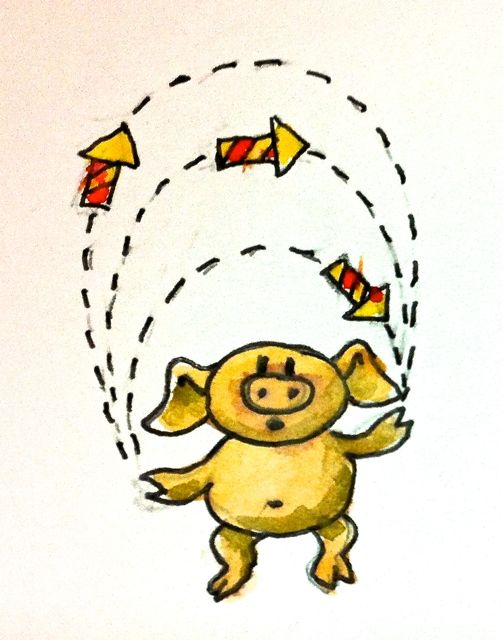
\includegraphics[width=2.45833in]{images/monoid.jpg}}
\end{figure}

String concatenation is an interesting case, because we have a choice of
defining right appenders and left appenders (or \emph{prependers}, if
you will). The composition tables of the two models are a mirror reverse
of each other. You can easily convince yourself that appending ``bar''
after ``foo'' corresponds to prepending ``foo'' after prepending
``bar''.

You might ask the question whether every categorical monoid --- a
one-object category --- defines a unique set-with-binary-operator
monoid. It turns out that we can always extract a set from a
single-object category. This set is the set of morphisms --- the adders
in our example. In other words, we have the hom-set \texttt{M(m, m)} of the
single object \texttt{m} in the category \texttt{M}. We can easily define a binary
operator in this set: The monoidal product of two set-elements is the
element corresponding to the composition of the corresponding morphisms.
If you give me two elements of \texttt{M(m, m)} corresponding to \texttt{f} and
\texttt{g}, their product will correspond to the composition
\texttt{g∘f}. The composition always exists, because the source and the
target for these morphisms are the same object. And it's associative by
the rules of category. The identity morphism is the neutral element of
this product. So we can always recover a set monoid from a category
monoid. For all intents and purposes they are one and the same.

\begin{figure}
  \centering
          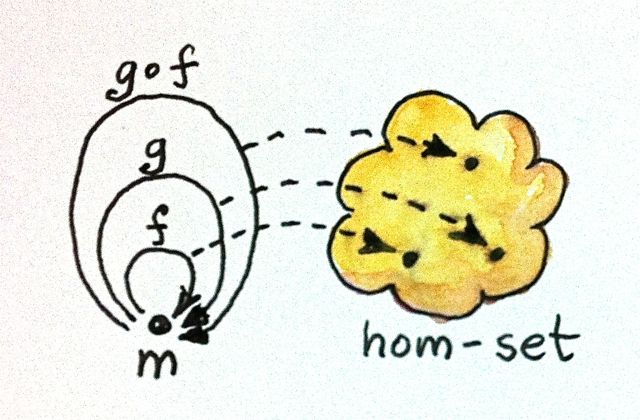
\includegraphics[width=3.12500in]{images/monoidhomset.jpg}
      \captionsetup{labelformat=empty,font=scriptsize}
      \caption{Monoid hom-set seen as morphisms and as points in a set.}
\end{figure}

There is just one little nit for mathematicians to pick: morphisms don't
have to form a set. In the world of categories there are things larger
than sets. A category in which morphisms between any two objects form a
set is called locally small. As promised, I will be mostly ignoring such
subtleties, but I thought I should mention them for the record.

A lot of interesting phenomena in category theory have their root in the
fact that elements of a hom-set can be seen both as morphisms, which
follow the rules of composition, and as points in a set. Here,
composition of morphisms in M translates into monoidal product in the
set \texttt{M(m, m)}.

\subsection{Acknowledgments}\label{acknowledgments}

I'd like to thank Andrew Sutton for rewriting my C++ monoid concept code
according to his and Bjarne Stroustrup's latest proposal.

\subsection{Challenges}\label{challenges}

\begin{enumerate}
\item
  Generate a free category from:

  \begin{enumerate}
  \item
    A graph with one node and no edges
  \item
    A graph with one node and one (directed) edge (hint: this edge can
    be composed with itself)
  \item
    A graph with two nodes and a single arrow between them
  \item
    A graph with a single node and 26 arrows marked with the letters of
    the alphabet: a, b, c \ldots{} z.
  \end{enumerate}
\item
  What kind of order is this?

  \begin{enumerate}
  \item
    A set of sets with the inclusion relation: A is included in B if
    every element of A is also an element of B.
  \item
    C++ types with the following subtyping relation: T1 is a subtype of
    T2 if a pointer to T1 can be passed to a function that expects a
    pointer to T2 without triggering a compilation error.
  \end{enumerate}
\item
  Considering that Bool is a set of two values True and False, show that
  it forms two (set-theoretical) monoids with respect to, respectively,
  operator \texttt{\&\&} (AND) and \texttt{\textbar{}\textbar{}} (OR).
\item
  Represent the Bool monoid with the AND operator as a category: List
  the morphisms and their rules of composition.
\item
  Represent addition modulo 3 as a monoid category.
\end{enumerate}